\documentclass{article}
\usepackage{graphicx}
\usepackage[utf8]{inputenc}
\usepackage{fullpage}
\usepackage{enumitem}
\usepackage{hyperref}
\usepackage{titling}
\usepackage{mathtools}

\parindent0in
\pagestyle{plain}
\thispagestyle{plain}

\newcommand{\myname}{John Doe}
\newcommand{\assignment}{Práctica SVM}
\newcommand{\duedate}{27 de Noviembre, 2018}

\renewcommand\thesubsection{\arabic{subsection}}

\title{Support Vector Machine}
\author{Erick Tornero}
\date{}

\begin{document}

Universidad Católica San Pablo\hfill\\
Sistemas Inteligentes\hfill\textbf{\assignment}\\
Prof.\ José Ochoa, Graciela Mesa\hfill\textbf{Entrega:} \duedate\\
\smallskip\hrule\bigskip

{\let\newpage\relax\maketitle}
% \maketitle

\section{Preguntas de Teoría:}

\begin{itemize}
    \item [6] Demuestre la primera condición de \textnormal{KKT}, i.e: 
    \[
        \frac{\partial \mathcal{L}}{\partial w} (\omega^*, b^*, \alpha)= \omega^* - \sum_{i=1}^m \alpha_i y(i)x^{(i)}    
    \]
    
Sea el conjunto $N = \{((1, 6), -1), ((4, 9), -1),((4, 6), -1), ((5, 1), 1), ((9,5), 1), ((9,1), 1), ((0, 3), 1),$ \newline
$((2,2),-1), ((3,1),-1)\}$ y el
hiperplano $H_1$ definido anteriormente


    \item [9] Calcule la holgura de los ejemplos no separables.

    Sean los ejemplos no separables y los puntos: $M1 = \{((0, 3), 1), ((2,2),-1), ((3,1),-1)\}$, y el hiperplano $H1$: $H_1: x1 - x2 - 1 = 0$
    Se define la $holgura \xi$:
    \[
        y_i(<\omega, x_i> + b) \geq 1 - \xi_i, \xi_i \geq 0, i = 1,\dots, n    
    \]

    Cálculo de $\xi_1$: $-4 \geq 1 - \xi_1$ $\Rightarrow \xi_1 = 5$

    Cálculo de $\xi_2$: $1 \geq 1 - \xi_2$ $\Rightarrow \xi_2 = 0$

    Cálculo de $\xi_3$: $-1 \geq 1 - \xi_3$ $\Rightarrow \xi_3 = 2$ 


    \section{Preguntas de Investigación}

    \item [11] Describa el significado del parametro $\gamma$ en el kernel gaussiano. Luego, explique la influencia de $\gamma$ en la
    capacidad de generalización de una SVM.

    Sea el Kernell Gaussiano: $exp( \frac{- \Vert x - x' \Vert^2}{2\sigma^2}) with \gamma > 0$
    
    Se define $\gamma = \frac{1}{\sigma^2}$, por tanto: 

    $exp(-\gamma \Vert x - x' \Vert^2) with \gamma > 0$

    Ya que El kernell Gaussiano es un Kernell Radial, la varianza de este Kernell dado por $\sigma^2$, 
    representa el grado de ajuste a los datos, esto quiere decir que una varianza pequeña, implica que
    habra un sobreajuste a los datos particulares, en cambio una varianza más grande implicara mayor 
    grado de generalización, el término $\gamma$ implica lo contrario, se escoger un $\gamma$ lo suficientemente
    pequeño para lograr una buena generalizacion y a su vez un $\gamma$ lo sificientemente grande para lograr
    un ajuste adecuado.

    \section{Implementación}

    \item [13] Experimente y muestre resultados usando diferentes valores para los parámetros de los kernels: lineal,
    polinomial, gaussiano, y el parámetro $C$.

    Resultado de clasificar con kernels \textit{lineal, polinomial y gaussiano}. Ver \ref{PLOT_P1_3}
    \begin{figure}[h]
        \label{PLOT_P1_3}
        \centering
        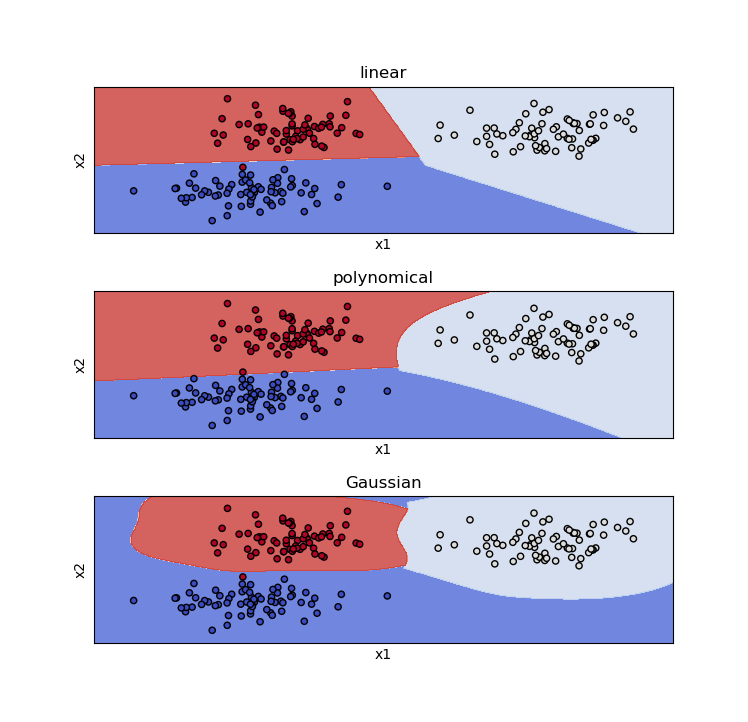
\includegraphics[width=.6\textwidth]{graphics_data1.png}
        \caption{C = 1.0}
    \end{figure}
     
    Variando los valores de $C$ para un \textit{Kernell polinomial}, se observa
    que el clasificador acepta más valores cuando el valor de $C$ es más pequeño, ya que le otorga
    más flexibilidad con el error, ver pregunta teórica 1, lo contrario ocurre cuando
    el valor de $C$ incrementa. Ver Figura \ref{PLOT_C_V}
    \begin{figure}[h]
        \label{PLOT_C_V}
        \centering
        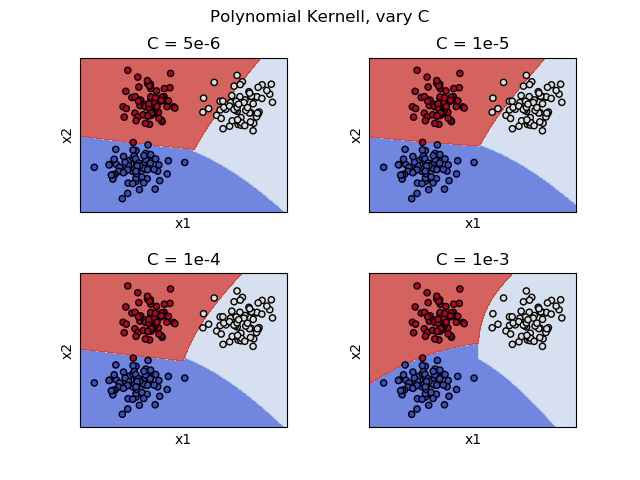
\includegraphics[width=.6\textwidth]{variance_c.png}
        \caption{Lineal, Pol: C = 0.01, Gaussiano: C=0.03}
    \end{figure}

    Variando los valores de $\gamma$ para un \textit{Kernell Gaussiano, con C = 10.0}, se observa una mejor
    generalización para valores bajos de $\gamma$, puede observarse un sobreajuste a medida que
    se incrementa el valor de $\gamma$, este comportamiento es explicado en la pregunta 2
    de las \textit{preguntas de Investigación}. Ver figura \ref{PLOT_G_V}.
    
    \begin{figure}[h]
        \label{PLOT_G_V}
        \centering
        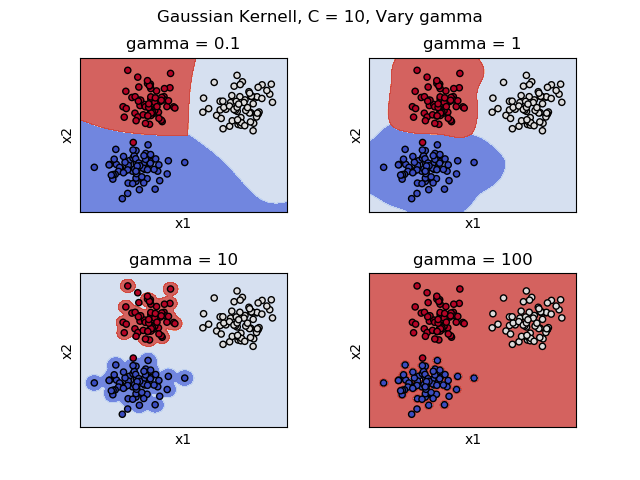
\includegraphics[width=.6\textwidth]{variance_gamma.png}
        \caption{Lineal, Pol: C = 0.01, Gaussiano: C=0.03}
    \end{figure}


    Resultado de clasificar con kernels \textit{lineal, polinomial y gaussiano}. Ver \ref{PLOT4}, para valores de $C$ bajos
    es decir con alta flexibilidad, se puede observar esto fuertemente en el kernel gaussiano.
    \begin{figure}[h]
        \label{PLOT4}
        \centering
        \includegraphics[width=.6\textwidth]{graphics_dataC.png}
        \caption{Lineal, Pol: C = 0.01, Gaussiano: C=0.03}
    \end{figure}


\end{itemize}
\end{document}